\subsection{Example of an application in social network analysis}
\label{sec:applications}

We conclude this section on experiments with a small example 
demonstrating the application of the clique algorithms for detecting overlapping communities in social networks. 
In many real networks vertices may belong to more than one group, and such groups form overlapping communities. Classical examples are social networks, where an individual usually belongs to different circles at the same time, from that of work colleagues to family, sport associations, etc. 
Finding overlapping communities is a challenging problem \cite{Fortunato_2010}.
Clique algorithms are one way in which a solution can be found.  
%A detailed overview of community detection methods, and the significance and complexity involved in overlapping community findingcan be found in \cite{Fortunato_2010}.

%\vspace{-20pt}
\begin{figure}%[h!]
  \centering
    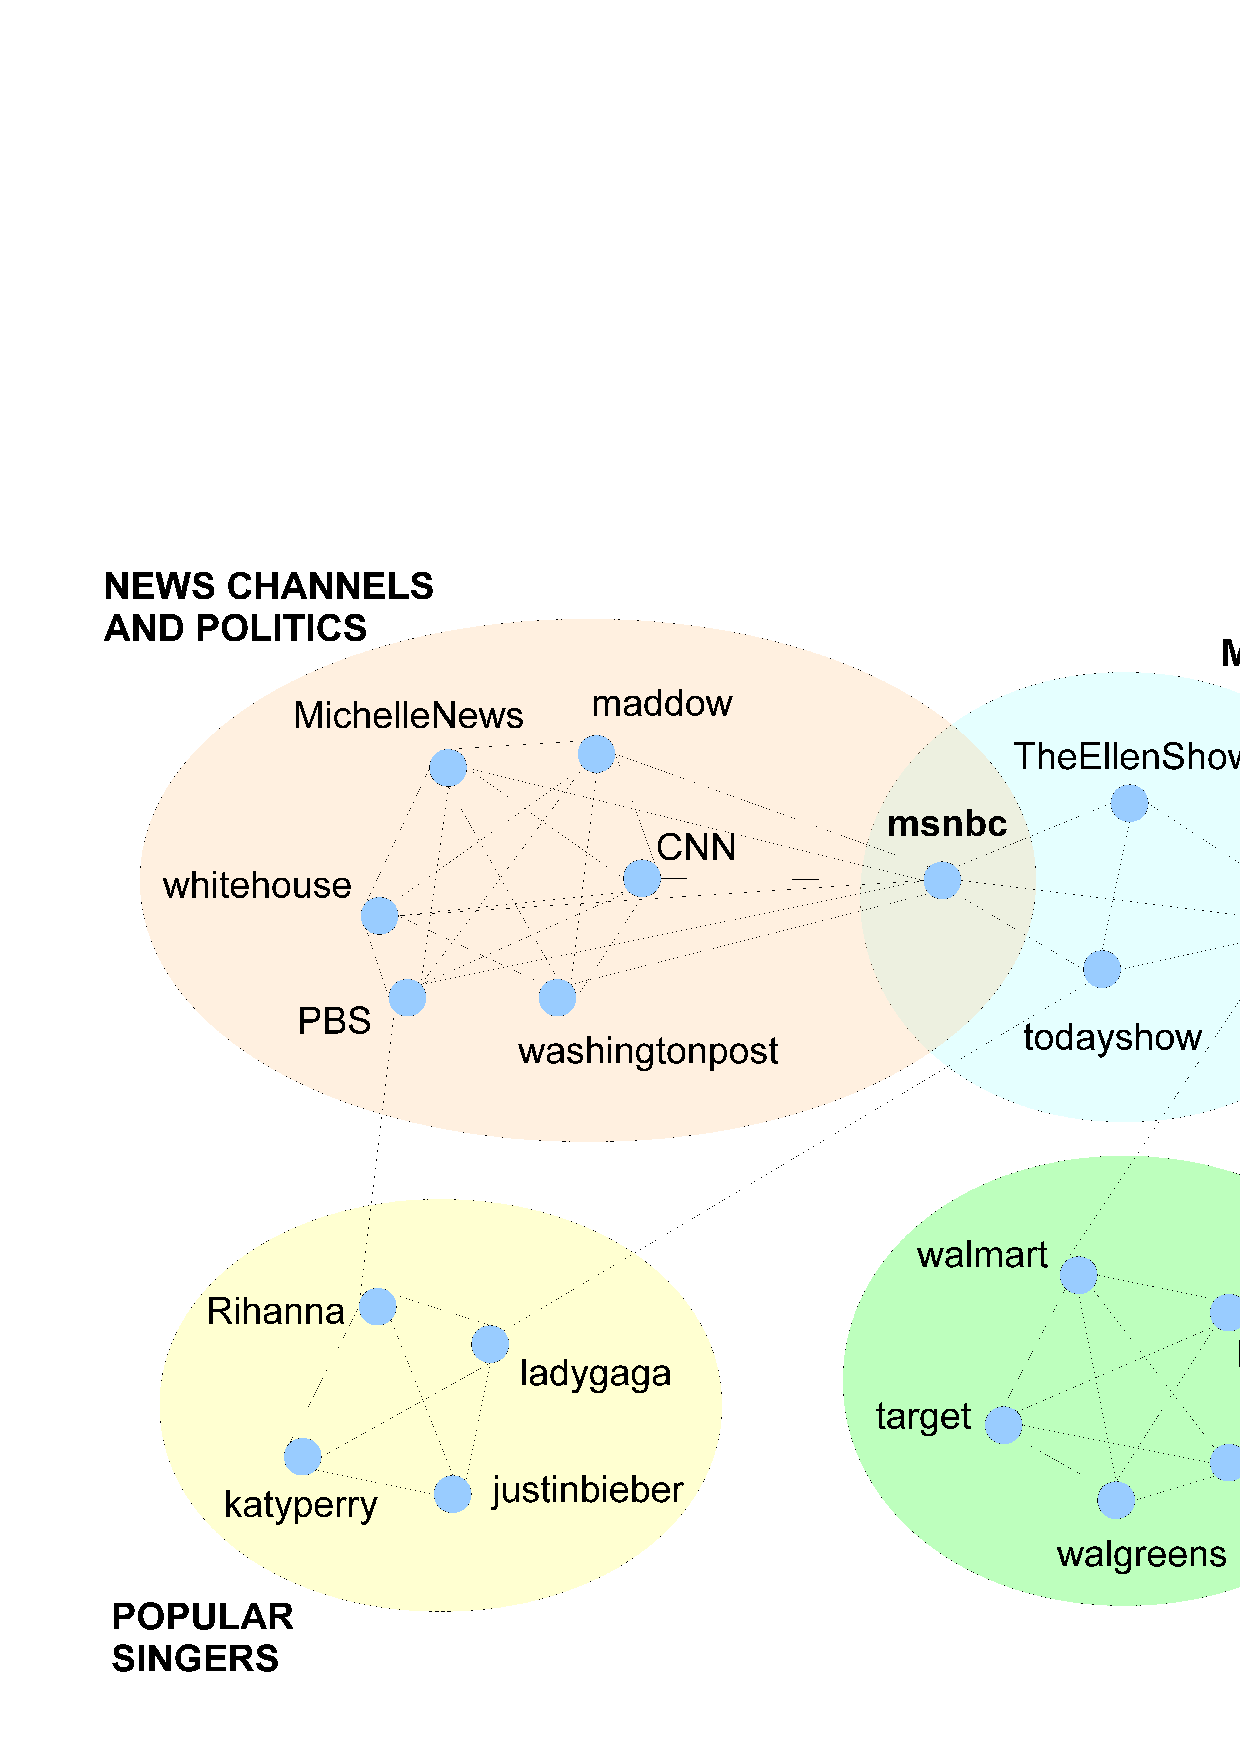
\includegraphics[width=1\textwidth]{communities.pdf}
%\vspace{-30pt}
  \caption{Some Facebook communities detected by our max clique heuristic.}
\label{fig-communities}
\end{figure}
%\vspace{-10pt}

%\footnotetext{http://www.facebook.com}
For our small experiment, we use data collected from Facebook\footnote[1]{http://www.facebook.com}.
Every user on Facebook has a {\it wall}, which is a the user's profile space that allows the posting of messages, often short or temporal notes by other users. The user comments and user information from specific {\it walls} are publicly available and we collected them using Facebook API. We constructed a graph with the {\it walls} as vertices. Any two users who have commented on the same {\it wall} indicate a connection between the {\it walls}, and we form an edge between them. There could be many common users for each wall, and so we assigned edge weights by Jacard index or similarity coefficient \cite{Leydesdorff}. Once this is done for all {\it walls}, we retained only those edges which have weights above a chosen threshold, indicating a strong correlation. The threshold is a user's choice and decides both the size and the number of communities found.
% If an edge already exists, we increase the edge weight by 1. Once this is done for all {\it walls}, the edge weights are normalized, and we retain only those edges which have edge weights above a chosen threshold (we use 0.01), indicating a strong correlation.

%duplicate removal
We modified our heuristic to retain the largest maximum clique containing each node. 
%This is done by simply substituting Lines 3 and 4 of Algorithm \ref{alg:clqHeu}, with a simple routine that stores each clique in a preferred data structure. 
The exact algorithm could have also been used instead of the heuristic for this purpose. We choose the heuristic since it is much faster and for this particular problem of community detection the accuracy of the size of cliques formed is not critical.

Figure \ref{fig-communities} shows some of the cliques/communities detected. We see two isolated communities, one for popular singers, and another for retail chains and products. We also see a community for news channels and politics, and a community of MSNBC and popular TV shows. The highlight of this experiment  is that the
clique algorithm allows a node to be a member of more than one community giving an overlapping community structure. Although the {\it news channels and politics} and {\it MSNBC and tv shows} communities are not directly related and have different members, they share a common member.
%add from nature paper why this is significant. coexistence of their structural subunits 

